\section{Proposed Feature-based Transfer Learning Models}
Obtaining the above features for link and time,
we first apply several classic machine learning models for regression that are trained on source areas with above-explored spatiotemporal features and then simply predict traffic condition on target areas as a test.
Afterwards, we present a novel transfer learning approach named CTMP.

\textit{Notations:} a prediction query instance about a link $l$ at the time $t$ is denoted as $(l,t)$; 
the spatial feature vector for the link $l$ is denoted as  $s_l$, and the temporal feature vector of the time $t$ being predicted on the link $l$ is denoted as  $t_l$.
The ground truth of the speed is denoted as $v_l[t]$.
\subsection{Linear Regression Model}
Linear regression (LR) is an approach for modeling the relationship between a scalar dependent variable $y$ and one or more explanatory variables denoted $\mathbf x$. 
%The linear regression method is a typical supervised learning method since $\mathbf x$ and $y$ are all known and the relationships are modeled using linear predictor functions whose unknown model parameters are estimated from the data. 
The model can be expressed in the following form:
$y = \mathbf{w}^T \mathbf{x} + b$ ,where $w$ and $b$ are the parameters we should learn in order to optimize a particular loss. 
%Many methods can be adopted, such as the gradient descent method, to find the proper parameter of the linear model.
In our case, we regard the $\mathbf x$ for each query instance as the concatenation of the spatial feature $s_l$ and the temporal feature $t_l$. 
Thus, we have $\mathbf{x} = [s_l;t_l]$.



\subsection{Neural Network Model}
%Neural network is a kind of computational model widely used in 
%machine learning, computer science and other research disciplines. 
%Recent research indicates that traditional machine learning methods are not sufficiently capable of extracting suitable features and capturing the non-linear nature of complex tasks. 
%Neural network models are presented as a remedy. 
%Fig. \ref{fig:nn} shows the structure of a typical three-layer neural network. 
%Each connection between (two) neurons can transmit an unidirectional signal with an activating strength that varies with the strength of the connection. 
%As a result, a typical four-layer neural network model can approximate most non-linear functions.
%
We adopt a four-layer neural network model (MLP) with following structure: 
the size of input layer is equal to the dimensionality of $\mathbf{x}$; 
the second layer contains half of it; 
the third is half of the second layer; 
the final output layer contains only one neuron.
The model (NN) takes the same input as before and output a continuous value by the last output layer which is the predicted speed.
%If the combined incoming signals (from potentially many transmitting neurons) are strong enough, the receiving neuron activates and propagates a signal to downstream neurons connected to it.

%\begin{figure}[th!]
%	\centering
%	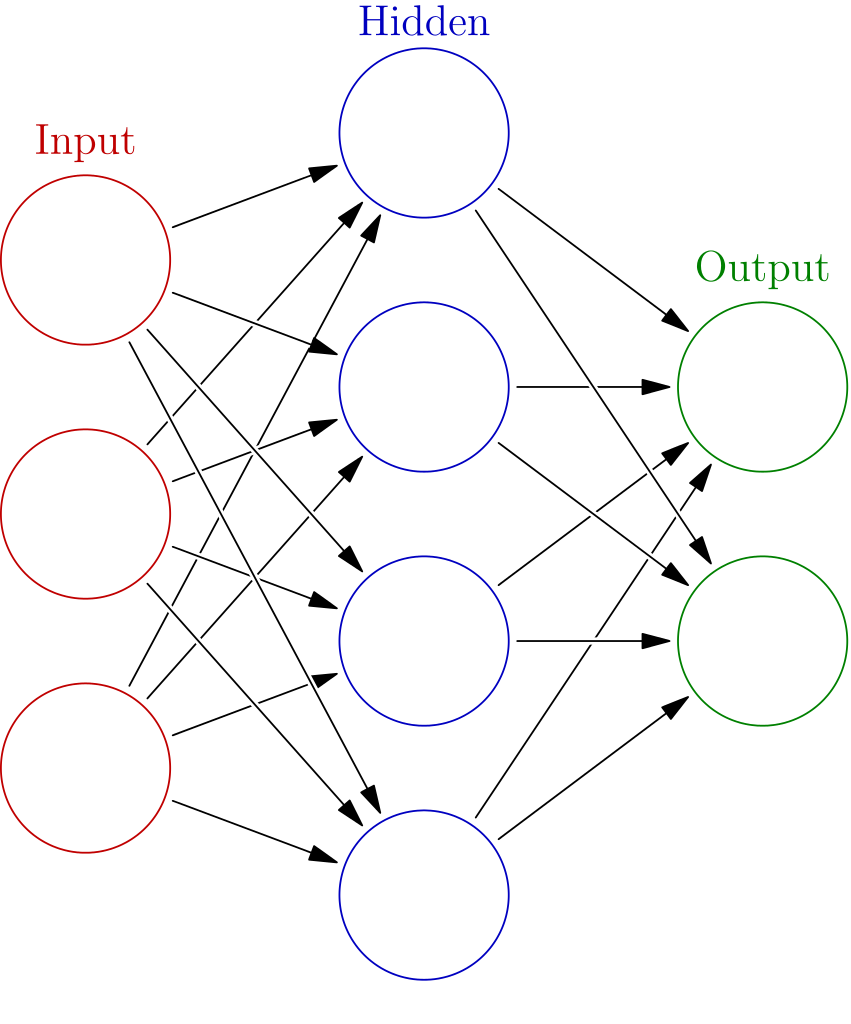
\includegraphics[width=0.3\textwidth]{figures/Colored_neural_network.png}
%	\caption{Structure of a typical neural network}
%	\label{fig:nn}
%\end{figure}

%Moreover, a threshold may govern each connection and neuron, such that the signal must exceed the limit before propagating. 
%Back propagation is the use of forward stimulation to modify connection weights. 
%Training typically requires several thousand cycles of interaction.
%
%In our work, we ...

\subsection{Support Vector Regression Model}
Support vector regression (SVR) depends only on a subset of the training data, 
because the cost function for building the model ignores any training data close to the model prediction. 
Training the original SVR means solving following optimization problem, where ${\displaystyle \mathbf{x_{i}}}$ is a training sample with target value ${\displaystyle y_{i}}$:
\begin{align*}
\min ~ {\displaystyle {\frac {1}{2}}\|\mathbf{w}\|^{2}}, ~~
\text{subject to} ~{\displaystyle {\begin{cases}y_{i}-\langle \mathbf{w},\mathbf{x_{i}}\rangle -b\leq \varepsilon \\\langle \mathbf{w},\mathbf{x_{i}}\rangle +b-y_{i}\leq \varepsilon \end{cases}}}
\end{align*}

%The inner product plus intercept ${\displaystyle \langle w,x_{i}\rangle +b} $
%is the prediction for that sample,
%and ${\displaystyle \varepsilon }$  
%is a free parameter that serves as a threshold: 
%all predictions have to be within an ${\displaystyle \varepsilon }$ 
%range of the true predictions. Slack variables are usually added into the above to allow for errors and to allow approximation in the case the above problem is infeasible.


%To predict the future traffic speed, we input spatial and temporal features as x and the true traffic speed as y for training. 
%After obtaining the $w$ and $b$, we use this model to predict traffic speed of test data and compare the prediction with true data. 

%\subsection{CTMP: A Clustering-based Transfer Model }
We introduce our novel \textbf{C}lustering-based \textbf{T}ransfer \textbf{M}odel for \textbf{P}rediction  (CTMP), which first clusters links in both source and target areas based on their spatial features and then do time series based prediction for the target links based on neighboring source links with historical data.

\subsection{Intuition Behind the CTMP}
Our intuition behind CTMP is that given a link in target areas with spatial features, we can first find the most similar links in source areas and then leverage the source data to predict the speed of links in target areas.

The assumption here is that links with similar spatial features should also share similar traffic patterns.
However, simply clustering road links based on spatial features performs not very well in practice, because not all the features are equally important and the importances cannot be obtained in such an unsupervised way.
Therefore, we incorporate a regularization term in the distance metric for feature reduction and selection.\footnote{CTMP model can be seen as a combination of clustering and Nadaraya-Watson kernel regression.}

\subsection{Clustering with Regularized Distance Metric}
%\textit{Notations:} a prediction query instance about a link $l$ at the time $t$ is denoted as $(l,t)$; 
%the spatial feature vector for $l$ is denoted as  $s_l$, and the temporal feature vector of the time $t$ being predicted on the link $l$ is denoted as  $t_l$.
%The ground truth of the speed is denoted as $v_l[t]$.
We use the $s_i$ and $s_j$ to denote two spatial feature vectors of any two links $i$ and $j$ respectively.
We capture the distance between the two feature vectors by computing $\text{s\_dis}(i,j) = 1-\cos(s_i,s_j)$.
To regularize the time series similarities between two links, we add a regularization term $\text{t\_dis}(i,j)$, which has multiple options.
A desirable option is the DTW \cite{} similarities between the weekly HAM traffic speed series of the two links.
Thus, the total distance between two links can be regarded as follows, where $\lambda$ is a hyper parameter to control the weight of temporal distance:
$\text{dis}(i,j) =  \text{s\_dis}(i,j) + \lambda \text{t\_dis}(i,j) $.

With such supervision in the source area data,
we can use K-means as our clustering algorithm.
For each query instance $(l,t)$\footnote{The link $l$ has no historical data in the transfer scenario.}, we first find the closest $k$ neighboring source links with historical data $\{l_1,...l_k\}$.
We compute all the distances between them and the target link $l$ respectively, and obtain the set of spatial feature distances $\{\text{dis}(l,l_1),...,\text{dis}(l,l_k)\}$.
Also, we can get the predicted typical traffic speed for such neighboring links based on existing time-series models  at the time $t$: $\{y(l_1,t),...,y(l_k,t)\}$.
Finally, we can compute the predicted result for the query instance $(l,t)$ is:
$$ y(l,t) = \sum_{i=1}^k \left( \frac{\text{dis}(l,l_i)}{\sum_{j=1}^k \text{dis}(l,l_j)} 
y(l_i,t)
\right)$$ 

%\BL{add a figure to illustrate this novel model}